% Compile from this directory: pdflatex report.tex (twice).
% Replace the three author placeholders before submission.
\documentclass[10pt,a4paper]{article}
\usepackage[T1]{fontenc}
\usepackage[utf8]{inputenc}
\usepackage{lmodern,textcomp}
\usepackage[margin=23mm]{geometry}
\usepackage{amsmath,amssymb,booktabs,tabularx,array,longtable}
\usepackage{graphicx,pdflscape,microtype,xcolor}
\usepackage[hidelinks]{hyperref}
\hypersetup{pdftitle={Assignment 2: Business Process Analysis and Redesign},pdfauthor={Student group}}
\newcommand{\EUR}{\texteuro}
\newcommand{\StudentOne}{[Student 1: name and student ID]}
\newcommand{\StudentTwo}{[Student 2: name and student ID]}
\newcommand{\StudentThree}{[Student 3: name and student ID]}
\newcolumntype{Y}{>{\raggedright\arraybackslash}X}
\setlength{\parindent}{0pt}
\setlength{\parskip}{5pt}
\setlength{\emergencystretch}{2em}
\renewcommand{\arraystretch}{1.15}
\title{\textbf{Assignment 2: Business Process Analysis and Redesign}\\[4pt]
\large IT Helpdesk: As-Is Analysis, Staffing and To-Be Design\\[3pt]
\normalsize INFO-H420 --- Process Modeling, Data Pipelines, and Responsible AI}
\author{\StudentOne\\\StudentTwo\\\StudentThree}
\date{}
\begin{document}
\maketitle
\begin{abstract}
This report analyzes the supplied IT-helpdesk process and presents a possible redesign.
The analytical as-is cycle-time efficiency is 4.742\%, with a processing labor cost of
\EUR176.67 per execution under Exercise 1's handoff exclusion. An Erlang-C calculation
requires three Level-2 employees for a two-hour resolution service at one request per
hour; including evaluation and writing in a single service visit requires four.
At the four-request-per-hour workload of Exercise 3, three Level-2 employees are
insufficient. A 12-configuration simulation identifies the capacity bottleneck and
diminishing returns beyond approximately 12 Level-2 employees. Six issues are linked
to redesign proposals. The selected to-be model automates routine delivery and
feedback routing while retaining human assistance. At matched staffing, the main
redesign run reduces modeled labor cost per case by approximately 7\%; its smaller
cycle-time change requires more cautious interpretation.
\end{abstract}

\subsection*{Scope and modeling conventions}
The assignment describes five Level-1 employees at \EUR40 per person-hour and three
Level-2 employees at \EUR60 per person-hour, serving approximately 500 company
employees~\cite{assignment}. Each staffed activity requires \emph{one} employee.
The capacity of three is a shared pool, not a three-person team per request.

The supplied BPMN model is used for Exercises 1 and 3. Known requests occur with
probability 0.2; otherwise the request is escalated. Each delivered Level-2 resolution
succeeds with probability 0.8. Unsuccessful cases return to resolution work, not to
initial evaluation. Repeated outcomes are modeled as independent with unchanged
probabilities. No business-hour calendar is imposed because the assignment provides
no shift schedule. All reported hours are continuous modeled hours unless explicitly
identified as working hours in the queueing calculation.

\section{Exercise 1: cycle-time efficiency and cost per execution}
\subsection{Expected activity visits}
Let $p=0.8$ denote the probability of escalation and $r=0.2$ the probability that a
resolution fails. Conditional on escalation, the number of resolution attempts $N$
is geometrically distributed:
\[
 \mathbb{E}[N\mid\text{escalated}]=\frac{1}{1-r}=1.25.
\]
Consequently, each activity in the resolution--delivery--feedback loop is visited
$p/(1-r)=1$ time per incoming request on average. Initial evaluation is visited
$0.8$ times; forwarding unsuccessful feedback is visited $pr/(1-r)=0.2$ times.
The known-resolution branch is visited $0.2$ times.

\begin{table}[htbp]
\centering\small
\caption{As-is inputs and expected visits. Durations are minutes per visit.}
\label{tab:asis-inputs}
\begin{tabularx}{\linewidth}{Ylrrr}
\toprule
Activity & Resource & Work & Delay & Visits/case\\
\midrule
Check request & Level 1 & 10 & 60 & 1.0\\
Send known resolution & Level 1 & 5 & 0 & 0.2\\
Evaluate request & Level 2 & 20 & 120 & 0.8\\
Solve request & Level 2 & 120 & 1200 & 1.0\\
Write resolution & Level 2 & 20 & 0 & 1.0\\
Send written resolution & Level 1 & 20 & 1200 & 1.0\\
Receive client response & None & 0 & 1200 & 1.0\\
Forward unsuccessful feedback & Handoff & 0 & 2 & 0.2\\
\bottomrule
\end{tabularx}
\end{table}

Exercise 1 explicitly excludes waiting and handoffs from processing time and cost.
Accordingly, the two-minute forwarding step is excluded from labor but retained as
elapsed handoff time. In BpmnGo this is represented by zero processing time and a
two-minute unresourced delay. This is an accounting convention for Exercise 1,
not a claim that forwarding physically requires no work.

\subsection{Processing time and cycle time}
Expected actual-work time per request is
\begin{align*}
 T_{L1} &= 10+0.2(5)+1(20)=31\text{ min},\\
 T_{L2} &= 0.8(20)+1(120)+1(20)=156\text{ min},\\
 T_{\mathrm{work}} &=31+156=187\text{ min}.
\end{align*}
Expected waiting and elapsed handoff time is
\[
 T_{\mathrm{delay}}=60+0.8(120)+1200+1200+1200+0.2(2)
 =3756.4\text{ min}.
\]
The configured 20-hour waits before resolution work and delivery apply on each
visit through the corresponding loop activities. Thus,
\[
 T_{\mathrm{cycle}}=187+3756.4=3943.4\text{ min}=65.723\text{ h},
 \qquad
 \mathrm{CTE}=\frac{187}{3943.4}\times100=\boxed{4.742\%}.
\]
The efficiency numerator follows the assignment's definition of actual work.
BpmnGo's value-added flags are configured to reproduce that definition; no separate
customer-value classification is inferred.

\subsection{Cost per execution}
Only actual processing labor is charged:
\[
 C=\frac{31}{60}(40)+\frac{156}{60}(60)
   =20.6667+156=\boxed{\text{\EUR176.67 per request}}.
\]
This is not the cost of employing the whole team for the request's elapsed cycle
time. The BpmnGo analytical calculation reproduced the values above. Given means
are sufficient for this calculation, so mean values were entered as fixed durations.

\section{Exercise 2: Level-2 staffing for a waiting-time target}
\subsection{Main queueing model}
The completed capacity calculation treats research and resolution as a single
Level-2 service station with mean service time two working hours. Requests reaching
this station arrive at rate $\lambda=1$ per working hour. An $M/M/c$ (Erlang-C)
model assumes Poisson arrivals, independent exponential service durations, identical
employees and a shared FIFO queue, without abandonment. These distributional
assumptions are additional to the assignment's stated means.

The service rate per employee is $\mu=1/2=0.5$ requests per hour. For $c$ employees,
let $a=\lambda/\mu=2$ and $\rho=a/c$. A stationary queue requires $\rho<1$.
The Erlang-C probability of waiting and mean queueing wait are
\begin{align*}
 P_W&=\frac{a^c/[c!(1-\rho)]}
 {\displaystyle\sum_{n=0}^{c-1}a^n/n!+a^c/[c!(1-\rho)]},&
 W_q&=\frac{P_W}{c\mu-\lambda}.
\end{align*}
With $c=2$, utilization is 100\% and no finite steady-state mean wait exists.
With $c=3$, $\rho=2/3$, $P_W=4/9$, and
\[
 W_q=\frac{4/9}{1.5-1}=\frac89\text{ h}=53.33\text{ min}<2\text{ h}.
\]
Therefore, \textbf{three Level-2 employees suffice under the two-hour
resolution-station interpretation}. The target concerns waiting before service,
not service plus waiting; the latter is $2.889$ hours at $c=3$.

\begin{table}[htbp]
\centering\small
\caption{Erlang-C results for one arrival per working hour.}
\begin{tabular}{lrrr}
\toprule
Service boundary & Service time (h) & Minimum staff & Mean wait (h)\\
\midrule
Research/resolution only & 2.000 & 3 & 0.889\\
Evaluation + resolution + writing, one visit & 2.667 & 4 & 0.757\\
\bottomrule
\end{tabular}
\end{table}

\subsection{Sensitivity to the service boundary}
If ``Level-2 service'' includes the initial 20-minute evaluation and 20-minute
writing task, one visit lasts $(20+120+20)/60=2.667$ hours. With the same $M/M/c$
approximation, three staff then yield $W_q=6.380$ hours; four yield $0.757$ hours.
This alternative excludes repeat visits. If one request per hour means \emph{new}
requests only, with rework generating additional visits, the arrival/workload model
must also account for that feedback. The two staffing answers therefore correspond
to different explicit service boundaries; the assignment's mean times alone do not
uniquely specify a queueing model.

\section{Exercise 3: simulation and resource experiments}
\subsection{Experiment design}
BpmnGo's discrete-event simulator was configured with constant Poisson demand at
four requests per hour, a 720-hour admission horizon, 20 replications, and initial
seed 42 (replication seeds 42--61). The system starts empty; no warm-up observations
are discarded. Resources are continuously available, use a common queue per pool,
and are released between activities. Individual staff identities are not retained
across a case's successive tasks.

All fixed internal waiting times in Table~\ref{tab:asis-inputs} are set to zero.
Only the client-response delay remains, as an unresourced 1200-minute wait.
Waiting for an occupied staff pool is generated by the simulation, not inserted
as another fixed delay. Forwarding unsuccessful feedback is modeled here as two
minutes of Level-1 work. Exercise 1's special handoff exclusion is not applied to
this operational simulation.

The known-resolution communication time follows a normal distribution with mean
5 and standard deviation 3 minutes; post-writing communication uses mean 20 and
standard deviation 5. Other processing durations are fixed at the supplied means.
BpmnGo resamples negative normal draws, so the realized mean of the short activity
is slightly higher than the nominal five minutes. This limitation also explains
small differences between simulated and analytical labor costs.

The baseline uses 5 Level-1 and 3 Level-2 staff. The factorial campaign compares
Level-1 capacities $\{3,5\}$ and Level-2 capacities $\{3,6,9,11,12,15\}$: 12
configurations, each with 20 replications. Two separate detailed runs retain the
baseline and the 5/12 configuration for resource-pressure comparison.

\subsection{Measured results}
\begin{table}[htbp]
\centering\small
\caption{Staffing experiment. Cycle times are hours; budget assumes the whole team
is paid continuously.}
\label{tab:staffing}
\begin{tabular}{rrrrrrr}
\toprule
L1 & L2 & Mean cycle & p95 cycle & Cases/h & Labor \EUR/case & Budget \EUR/h\\
\midrule
3 & 3 & 1,056.90 & 2,002.65 & 1.13 & 176.91 & 300 \\
3 & 6 & 316.63 & 715.45 & 2.20 & 176.41 & 480 \\
3 & 9 & 82.12 & 201.04 & 3.13 & 176.63 & 660 \\
3 & 11 & 25.69 & 54.71 & 3.61 & 177.22 & 780 \\
3 & 12 & 23.89 & 48.43 & 3.58 & 177.09 & 840 \\
3 & 15 & 23.39 & 46.74 & 3.59 & 177.16 & 1,020 \\
5 & 3 & 1,063.69 & 2,009.24 & 1.12 & 177.26 & 380 \\
5 & 6 & 321.12 & 720.36 & 2.18 & 177.55 & 560 \\
5 & 9 & 85.07 & 207.99 & 3.17 & 177.54 & 740 \\
5 & 11 & 25.42 & 54.14 & 3.63 & 177.06 & 860 \\
5 & 12 & 23.81 & 48.23 & 3.61 & 177.36 & 920 \\
5 & 15 & 23.15 & 46.19 & 3.61 & 176.69 & 1,100 \\
\bottomrule
\end{tabular}
\end{table}

The baseline mean cycle is 1063.69 hours, with an approximate 95\% confidence
interval of 1047.12--1080.26 hours across replication means. Level-2 utilization
is 97.37\%, its mean queue is 1166.92 requests, and the mean of per-replication
maximum queues is 1935. At 5/12, mean cycle falls to 23.81 hours (95\% interval
23.68--23.93 hours), Level-2 utilization is 78.32\%, and its mean queue falls to
2.25 requests. These metrics include the period after arrivals stop while the
remaining workload is drained.

\subsection{Interpretation and trade-offs}
The bottleneck can also be established analytically. Expected Level-2 work per
incoming request is 156 minutes, so at four arrivals per hour the offered workload is
\[
 a_{L2}=4\times\frac{156}{60}=10.4\text{ staff-hours per hour}.
\]
Three, six and nine Level-2 employees cannot sustain this workload. Eleven is the
smallest integer capacity strictly above it, but has little spare capacity.
The results show diminishing returns after approximately 12 Level-2 staff:
with five Level-1 staff, increasing Level-2 capacity from 12 to 15 saves about
39 minutes of mean cycle time while increasing the hourly staffing budget from
\EUR920 to \EUR1100.

Client feedback becomes dominant once staff queues are small. The expected number
of feedback waits per incoming request is $0.8/(1-0.2)=1$, contributing 20 hours.
With approximately 3.1 hours of work, the no-resource-queue analytical reference
is near 23.1 hours. Merely adding more employees cannot remove this external delay.

The 3/12 configuration gives a mean of 23.89 hours at \EUR840 per staffed hour,
compared with 23.81 hours and \EUR920 at 5/12. It is a candidate for further
assessment, not proof of equivalent service: the factorial output does not retain
an uncertainty interval for the difference, and no service-level target or budget
was specified. BpmnGo's selected 5/15 configuration minimizes mean cycle among the
tested points; it is not a demonstrated economic optimum.

\subsection{Metric limitations}
Every admitted case is drained to completion. Consequently, a completed campaign
does not imply a stable queue: the overloaded baseline is a finite-batch result,
not a steady-state waiting-time estimate. Throughput divides completions by elapsed
time through the final completion, and utilization uses the same extended period.
This explains why adequately staffed runs can report fewer than four completions
per hour. Counts are integer averages per replication, approximately 2869 cases,
not totals across all replications. Reported p95 values average per-replication
percentiles. Confidence intervals use $\bar{x}\pm1.96s/\sqrt{20}$.

Labor cost per case remains around \EUR177 because staffing mainly changes waiting,
not the amount of work. It excludes idle payroll. The separate budget measure is
$40c_{L1}+60c_{L2}$ per hour. Equal initial seeds improve reproducibility but do not
ensure identical case paths across configurations: changes in event order alter
random-draw consumption. Small differences in costs and paths should therefore
not be interpreted as redesign benefits.

\section{Exercise 4: issue register and redesign proposals}
The register in Table~\ref{tab:issues} distinguishes assignment assumptions from
simulation measurements. Severity and proposed responsibility are analyst judgments.
All six issues remain open: proposed interventions have not been deployed.
The fixed internal delays of Exercise 1 must not be counted again as gains in
Exercise 3, where they were explicitly removed.

\begin{table}[htbp]
\centering\small
\caption{Issue register.}
\label{tab:issues}
\begin{tabularx}{\linewidth}{@{}p{7mm}Y Y p{17mm}@{}}
\toprule
ID & Issue and evidence & Consequence / proposed owner & Severity\\
\midrule
I1 & Level-2 overload: workload is 10.4 staff-hours/hour; baseline mean queue is
1166.92 requests. & Unstable capacity at the original demand. Service desk manager. & High\\
I2 & Internal pickup delays: 1 h before checking, 2 h before evaluation, 20 h before
resolution and 20 h before delivery. & Expected contribution of 42.6 h per case in
Exercise 1. Workflow owner. & High\\
I3 & Level-1 relays a written resolution (20 min) and forwards failed feedback
(2 min). & Additional labor and transfers. Process owner. & Medium\\
I4 & Only 20\% are known at Level-1; 80\% are escalated. & 3.2 new Level-2
requests/hour before retries. Knowledge/training lead. & Medium\\
I5 & Each resolution fails with probability 20\%. & 1.25 attempts per escalated
request on average. Level-2 quality lead. & High\\
I6 & Client feedback takes 20 h per delivered resolution. & About 20 h of expected
cycle time per initial request. Client-service owner. & Medium\\
\bottomrule
\end{tabularx}
\end{table}

The following proposals apply the redesign heuristic terminology of Reijers and
Limam Mansar~\cite{reijers2005}. Their helpdesk-specific justification and test
plans are developed here.

\begin{description}
\item[C1 --- Extra resources (I1).]
Validate sufficient qualified Level-2 capacity, using 12 as a candidate under the
original workload. The measured 5/12 result directly addresses queue growth, but
raises the hourly staffing budget. Reassess capacity after changing work or routing;
additional employees should not substitute for analyzing unnecessary work.

\item[C2 --- Task automation (I2).]
Introduce event-driven assignment and notification to reduce avoidable pickup and
polling delay. First measure dispatch latency separately from capacity waiting:
the assignment does not identify how much of each stated delay is attributable to
batch handling rather than staff shortage. Use a separate timing sensitivity study
for the original fixed delays; an alert cannot remove a genuine resource queue.

\item[C3 --- Task elimination and task automation (I3).]
Deliver prepared resolutions automatically and route unsuccessful client feedback
directly to Level-2. Retain human assistance for cases requiring explanation.
This targets duplicate relaying rather than diagnosis. Test labor and cycle effects
at unchanged staffing and probabilities, and account for automation costs before
claiming financial savings.

\item[C4 --- Specialist--generalist (I4).]
Broaden Level-1 competence through targeted training and a maintained knowledge
base, retaining escalation for difficult cases. Test known/unknown probabilities
of 0.2/0.8, 0.3/0.7 and 0.4/0.6 as paired scenarios. With other assumptions fixed,
a 40\% known rate would reduce Level-2 workload to 7.8 staff-hours/hour. This is a
conditional calculation, not an observed improvement; training and additional
checking effort, and the risk of incorrect closure, must be included.

\item[C5 --- Control addition (I5).]
Add proportionate output validation before delivery. Test check durations of
0, 5 and 10 minutes together with explicitly hypothesized failure rates of
0.20, 0.15 and 0.10. Reduced rework may offset the extra effort, but checking can
also worsen an overloaded Level-2 queue. Validate quality and total labor, rather
than lowering the failure probability without paying for the proposed control.

\item[C6 --- Integration and task automation (I6).]
Provide direct test-result submission, clear instructions and proportionate
reminders. Test 20-, 10- and 5-hour client-response delays as sensitivity scenarios,
then measure actual behavior in a pilot. Client availability remains external to
the desk; silence must not be treated as successful resolution.
\end{description}

A practical sequence is to validate capacity, instrument dispatch, simplify the
relay, then pilot skill, quality and feedback improvements. C3 and C6 can share a
communication channel. Staffing must be recalculated after interventions change
workload. Six detailed entries, with evidence, heuristics, justification, trade-offs
and validation plans, were persisted in BpmnGo's issue register.

\section{Exercise 5: proposed to-be model and evaluation}
\subsection{Selected changes}
Figure~\ref{fig:tobe} implements a subset of C2, C3 and C6. The model preserves
request checking, the known-resolution branch, initial Level-2 evaluation, problem
solving and writing. A new exclusive gateway selects either automated notification
or Level-1 assisted delivery. Both paths merge before receiving the client's test
result. Confirmed successes close; failures are routed automatically back to the
merge before problem solving. Initial evaluation is not repeated.

The lanes separate Level-1 work, Level-2 work, and workflow automation/client-response
handling. The receive task represents the desk waiting for external feedback;
the client's internal testing process is outside the diagram. The design was
imported into BpmnGo's modeler, exported as editable BPMN, and saved as a separate
simulation project. Service-task symbols describe proposed integrations, not
already deployed notification or routing services.

\subsection{Additional assumptions and matched comparison}
The main scenario assumes 90\% of post-writing deliveries can be automated and
10\% require human assistance. This new probability is illustrative, not supplied
by the assignment. The assistance flag is assumed available without an additional
assessment task and is sampled at each delivery attempt. The assisted path retains
the original normal communication duration (mean 20 min, standard deviation 5 min).
Both automated tasks take one minute, require no human resource, and have zero
modeled incremental cost; development and operating costs remain unestimated.

Known/unknown probabilities remain 0.2/0.8, solved/rework probabilities remain
0.8/0.2, and client waiting remains 1200 minutes. No benefit from faster client
responses, better first-level resolution or fewer failures is assumed.
The primary as-is and to-be runs both use 5/12 staffing, four arrivals per hour,
720 hours, 20 replications and seed 42. Additional runs test 0\% and 100\%
automated delivery at 5/12 and 90\% automation at 5/3.



\subsection{Simulation results and interpretation}
\begin{table}[htbp]
\centering\small
\caption{As-is/to-be comparison and sensitivity checks. Cycle times are hours.}
\label{tab:tobe}
\begin{tabular}{llrrrr}
\toprule
Design & L1/L2 & Auto. delivery (\%) & Mean cycle & p95 cycle & Labor \EUR/case\\
\midrule
As-is & 5/12 & -- & 23.81 & 48.23 & 177.36 \\
To-be & 5/12 & 90 & 23.52 & 47.79 & 164.94 \\
To-be & 5/3 & 90 & 1,054.32 & 1,998.91 & 164.26 \\
To-be & 5/12 & 0 & 23.77 & 48.40 & 176.49 \\
To-be & 5/12 & 100 & 23.50 & 47.74 & 163.59 \\
\bottomrule
\end{tabular}
\end{table}

At matched 5/12 staffing, modeled labor cost falls from \EUR177.36 to \EUR164.94
per case, approximately 7.0\%. A simple expected-work check for 90\% automation is
\[
 C_{\mathrm{to\mbox{-}be}}
 =\frac{10+0.2(5)+0.1(20)}{60}(40)+\frac{156}{60}(60)
 \approx\text{\EUR164.67}.
\]
The simulation differs slightly because of stochastic routing and nonnegative-normal
sampling. Mean cycle changes from 23.81 to 23.52 hours, a difference of 17.0 minutes.
The approximate 95\% intervals are 23.68--23.93 hours and 23.34--23.71 hours;
they overlap. A separate uncertainty analysis of the difference is required before
asserting a statistically reliable cycle-time improvement.

The payroll budget remains \EUR920 per staffed hour in both 5/12 runs. The reduction
is in processing labor per case, not demonstrated payroll savings or a full
return-on-investment estimate. The zero-automation variant still routes failed
feedback automatically, so it is not identical to the original as-is process.

At 5/3, the to-be mean cycle is still approximately 1054 hours. Level-2 work remains
about 10.4 staff-hours per incoming hour; automation of the relay cannot resolve
that capacity shortage. Once adequate capacity is available, the retained 20-hour
client delay limits further elapsed-time improvement. The proposed design therefore
addresses avoidable relay work while preserving the need for a separate capacity
decision and evidence about automation coverage.

\subsection*{Overall assessment}
The original process combines a capacity bottleneck, repeated work and substantial
external waiting. Staffing changes have a large effect where capacity is inadequate;
process simplification reduces routine labor but does not replace specialist work.
The selected to-be model is a coherent proposal with explicit exceptions and
unchanged outcome probabilities. Its operational adoption would require validation
of automation coverage, communication quality, service targets and implementation
costs. The issue register remains open because simulation is evidence for a design
proposal, not confirmation of a production improvement.



\appendix
\section{Reproducibility and supporting files}
The local BpmnGo campaigns retain their input snapshots and run identifiers~\cite{bpmngo}.
The source package includes the following evidence in \texttt{data/}:
\begin{center}\small
\begin{tabularx}{\linewidth}{lY}
\toprule
Exercise & Supporting files\\
\midrule
1 & \texttt{exercise1-analysis.json}\\
2 & \texttt{exercise2-resolution.json}, \texttt{exercise2-full-visit.json}\\
3 & \texttt{exercise3-comparison.csv}, \texttt{exercise3-summary.json}\\
4 & \texttt{exercise4-register.json}\\
5 & \texttt{exercise5-comparison.csv}, \texttt{exercise5-summary.json}\\
\bottomrule
\end{tabularx}
\end{center}
The editable model is \texttt{helpdesk-to-be.bpmn}. All five Exercise 5 runs
completed with admitted and completed counts matching; the unchanged 5/12 run
reproduced Exercise 3's mean cycle and labor cost. Final model references and
parameters were checked. Reproduction requires the same engine behavior as well
as the same initial seed. Compile this report twice with pdfLaTeX, keeping the
\texttt{figures/} directory beside \texttt{report.tex}.

\begin{thebibliography}{9}
\raggedright
\bibitem{assignment}
INFO-H420 course materials.
\emph{Assignment 2: Business Process Analysis and Redesign}.
Provided assignment statement and accompanying BPMN model.

\bibitem{reijers2005}
H.~A. Reijers and S.~Limam Mansar.
``Best practices in business process redesign: an overview and qualitative evaluation
of successful redesign heuristics.''
\emph{Omega}, 33(4):283--306, 2005.
\href{https://doi.org/10.1016/j.omega.2004.04.012}{doi:10.1016/j.omega.2004.04.012}.

\bibitem{bpmngo}
BpmnGo local simulation laboratory.
Saved scenario snapshots, analytical outputs, issue register and simulation campaigns
for this assignment. Numerical evidence is included in the accompanying data files.
\end{thebibliography}
\clearpage
\begin{landscape}
\begin{figure}[p]
\centering
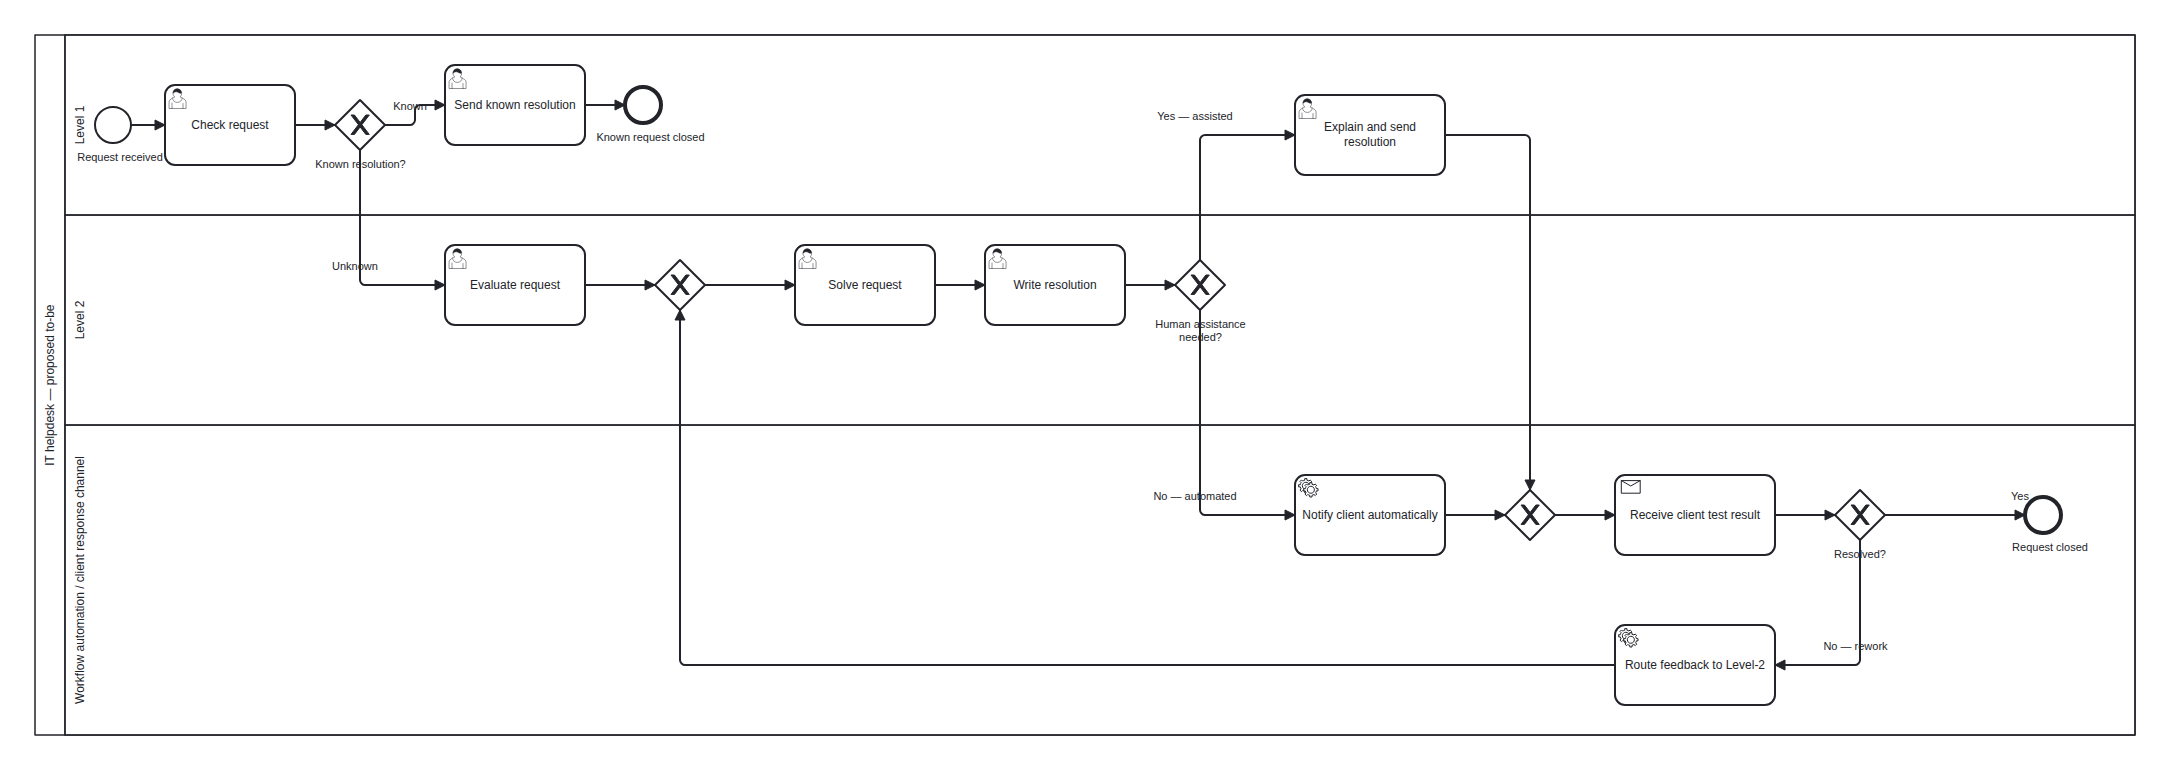
\includegraphics[width=\linewidth]{figures/to-be-diagram.png}
\caption{Proposed to-be helpdesk process. Routine delivery and unsuccessful-feedback
routing are automated, while a human-assisted delivery branch remains available.
The original success and escalation probabilities are preserved.}
\label{fig:tobe}
\end{figure}
\end{landscape}
\end{document}
